% HK to vet contributed texts
% 4.2 not written
% 4.3 onwards camera ready
\section{Neural Network Model}
\label{section_nn_model}

In this section, we first explain the input and structure of PubHRL, the neural network AlphaGeese is built upon. We explain how we attempted to improve the neural network model by changing the model architecture and the agents we train against. Finally we analyse some of the weakness of the neural network models.

\subsection{PubHRL Neural Network Model}
\label{section_pubhrl}

In this subsection, we explain the input and structure of PubHRL model \cite{notebook_pubhrl} to provide context to the improvements we attempt to make. The neural network model takes in a matrix of values, and returns four action-values and one state-value.

\subsubsection{Processing the Game State into the Model Input}
\label{subsection_pubhrl_input}

The PubHRL takes an input of a binary matrix of size (17,11,7). Each cell in the 11 $\times$ 7 game board is represented by 17 binary variables. Each "slice" of the matrix input encodes a different part of the information from the game board.

\begin{figure}[hb!]
\centering
  \includegraphics[width=0.6\linewidth]{images/input.png}
  \caption{Input block}
\end{figure}

\begin{itemize}
    \item The first four slices encode the position of the head, with one slice for each goose. The value in the matrix is 1 if the head belongs to the geese. Each slice is one-hot as there is at most one non-zero value. If the goose is dead, the slice will have values of all zeroes.
    \item The next four slices encode the position of the tail in a similar manner. Each slice of the tail encoding is one-hot.
    \item The next four slices encode the position of the body. The value in the matrix is 1 if the body belongs to the geese. These slices are not one-hot.
    \item The next four slices encode the position of the previous head position.
    \item The last slice encode the position of the food. 
\end{itemize}


% Each position the 11 \times 7 cells of each of the 17 "slice" represents the 2D positions of the game board and 17 represents the information encoded in the input. Hence, there are 17 slices of the game board that encode the different type of information from the observable data. Since there are four geese in the game, there will be four slices that encode the head, body, tail and previous head positions totaling to 16 slices. The last slice encodes the current position of the two foods. 

% This method of encoding the input is effective in transforming the observable data into a matrix form which is more suitable for deep learning model. 

There is sufficient information encoded in the input. The model can infer the length and shape of the goose from the position of the head, body and tail. Likewise, the direction of the previous move can be deduced from the difference between the position of the current head and the previous head. The input also takes into account the position of the other goose as well so that the goose can avoid colliding with them.

% The game provides all the observable information of the game environment at the current state to the agent. Information given are the exact position of the goose in the game board including the current placement of the food. Non-observable information such as where the next food is going to spawn is not given.

% discuss the merits of this encoding

\subsubsection{The Torus Block}
% to add - why the model is designed this way

The Torus Block consists of a two-dimensional convolution, ReLU and residual connections. A diagram of the architecture of the Torus Block can be seen as follows.

\begin{figure}[h!]
\centering
  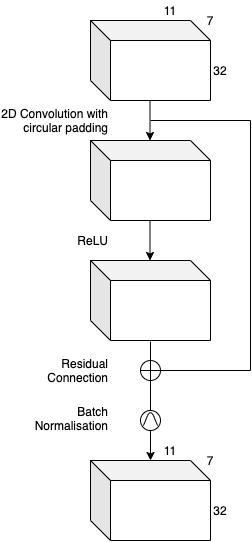
\includegraphics[width=0.4\linewidth]{images/torusblock-edit.png}
  \caption{Torus Block Architecture}
\end{figure}

The two-dimensional convolution uses filter size of 3 $\times$ 3 and has circular padding of size one to model the wrapping game board. The shape of the variables before and after the convolution is the same.

The output of the convolution is passed into ReLU. A non-linear function is used so that the neural can learn and produce a nonlinear decision boundary with non-linear combinations of the weight and inputs.

The output of ReLU is added with the input of the Torus Block. This summation is a residual connection and allows the model to address the vanishing gradient problem. In training, batch normalisation is also applied to improve gradient flow.

% is a piecewise linear function that outputs the input directly if positive, elsewise output zero. It is a favoured activation function because of its ease in calculation, and does not have a gradient vanishing. The Resnet layers create shortcut connections which control how much information from the past gets passed to the next time step. This help to train deeper models by addressing the vanishing gradient problem. 

\subsubsection{PubHRL Model Architecture}

The PubHRL model architecture is made up of Torus Blocks and fully connected layers.

\begin{figure}[h!]
\centering
  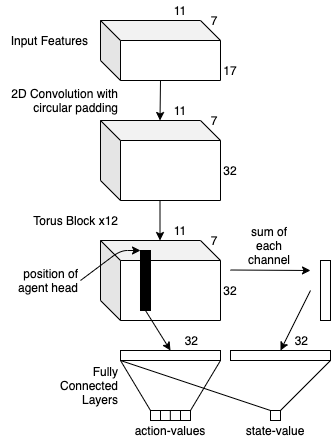
\includegraphics[width=0.6\linewidth]{images/pubhrl-edit.png}
  \caption{PubHRL Architecture}
\end{figure}

One convolution with circular padding transforms the input of size (17,11,7) to intermediate features of size (32,11,7). Then 12 Torus Blocks are applied on the intermediate features, which does not change the variable size of (32,11,7).

The values at the head position of the player's agent are extracted from the matrix, forming an array of size (1,32). The values at each of the 32 channels are summed, forming another array of size (1,32).

A fully connected layer transforms the values of the first array to the action-values. Another fully connected layer transforms the concatenation of the first and second array to the state-values. The fully connected layers are configured without bias.

This is how the model produces four action-values and one state-value. The model can be used directly to make inferences on which move to make, just by taking the action with the highest action-value.

% The PubHRL model is used to perform feature extraction based on the input data. The output is obtained in the advised next action and the resulting state value.

% The PubHRL model has 12 Torus Block Layers, in which the 32 features corresponding to a certain cell in the block is concatenated with the sum of each of 32 channels. The 64-bit value is then rearranged to output the advised next action and resulting state value.



% elaborate on the motivation behind the design on this model

\subsection{Dataset, Loss, and Training Architecture}
\label{subsection_dataset_and_training}
% HK still need to study what is going on.

As this is a reinforcement learning problem, dataset and loss functions are defined differently compared to supervised training. The objective of the training is to train the model to produce a good estimate of the policy-value and state-value.

The state-value $V^\pi(s)$ is the expected discounted return for a given state $s$ following policy $\pi$ that is assumed to be optimal. The action-value $Q^\pi(s,a)$ is the expected discounted return for taking action $a$ from a given state $s$ following policy $\pi$ that is assumed to be optimal \cite{blog_reinforcement_learning}.

As the number of possible game states is large, it is not possible to calculate the exact expectation for every state-value and action-value. Therefore state-value and action-value is approximated with a function, and the function is a neural network. The neural network is trained on squared loss \cite{blog_reinforcement_learning} between the predicted values and estimated values generated from the simulating the game.

One way to estimate the action-value and state-value without enumerating all possible states is to randomly simulate the actions until it reaches a terminal node in each complete episode. The payoff associated with the terminal node is backpropagated, thereby providing action-value and state-value for training. This method is known as the Monte Carlo (MC) method \cite{book_rl}.

It is possible to learn from incomplete episodes with Temporal Difference (TD) learning \cite{book_rl}. TD learning methods update targets with value estimates rather than solely relying on actual rewards from complete episodes as in MC methods. 

% Estimates are made with actors simulating the actions producing experience trajectories to learn from. The learner will use the experience trajectories to update the neural network parameters.
% last sentence I smoke one

It is possible to scale up training to achieve a very high throughput with the Importance Weighted Actor-Learner Architecture (IMPALA) framework \cite{paper_impala} \cite{blog_policy_gradient}. In the IMPALA framework, actors generate experience trajectories in parallel, while the learner optimizes the neural network parameters using generated experience. Actors update their parameters from the learner periodically. Because acting and learning are decoupled, we can generate many episodes with many actors in parallel and train the model more quickly. IMPALA also uses an off-policy gradient algorithm \cite{paper_off_policy} and TD learning to allow the decoupling and learning from past episodes for better sample efficiency and exploration \cite{blog_policy_gradient}.

HandyRL \cite{repo_handyrl} is an implementation of the IMPALA framework. We have used the training hyperparameters shared by PubHRL authors \cite{discussion_PubHRL_parameters}.

\subsection{Training Setup}
\label{subsection_training_setup}

The IMPALA framework allows the use of distributed computing resources to allow a high throughput for reinforcement learning training. For this to be possible, we need access to many virtual CPUs and a GPU. Therefore, we have trained our models on the Google Cloud Platform. Figure \ref{figure_training_setup} shows a screenshot of our training setup.


% [to paraphrase] HandyRL is a handy and simple framework based on Python and PyTorch for distributed reinforcement learning that is applicable to your own environments. HandyRL focuses on a practicable algorithm and implementation to create a strong and winning AI in competitive games. For large scale training, HandyRL provides a controllable high parallelism power according to your environment.

% [to paraphrase] HandyRL mainly provides a policy gradient algorithm with off-policy correction. From the perspective of stability and performance, the off-policy version policy gradient works fine in practice. So it’s a good first choice to create a baseline AI model. You can use some off-policy variants of update methods (targets of policy and value) from traditional ones (monte carlo, TD(lambda)) to novel ones (V-Trace, UPGO). These items can be changed in config.yaml.

% [to paraphrase] As a training architecture, HandyRL adopts a learner-worker style architecture like IMPALA. The learner is a brain of training which updates a model and controls the workers. The workers have two roles. They asynchronously generate episodes (trajectories) and evaluate trained models. In episode generation, self-play is conducted as default.

% [to paraphrase] In order to scale up RL training to achieve a very high throughput, IMPALA (“Importance Weighted Actor-Learner Architecture”) framework decouples acting from learning on top of basic actor-critic setup and learns from all experience trajectories with V-trace off-policy correction.

% [to paraphrase] Multiple actors generate experience in parallel, while the learner optimizes both policy and value function parameters using all the generated experience. Actors update their parameters with the latest policy from the learner periodically. Because acting and learning are decoupled, we can add many more actor machines to generate a lot more trajectories per time unit. As the training policy and the behavior policy are not totally synchronized, there is a gap between them and thus we need off-policy corrections.

% [to paraphrase] The underlying idea is that over time, the network will learn what states eventually lead to wins (or losses). In addition, learning the policy would give a good estimate of what the best action is from a given state. The neural network architecture in general would depend on the game

\begin{figure}[h]
\centering
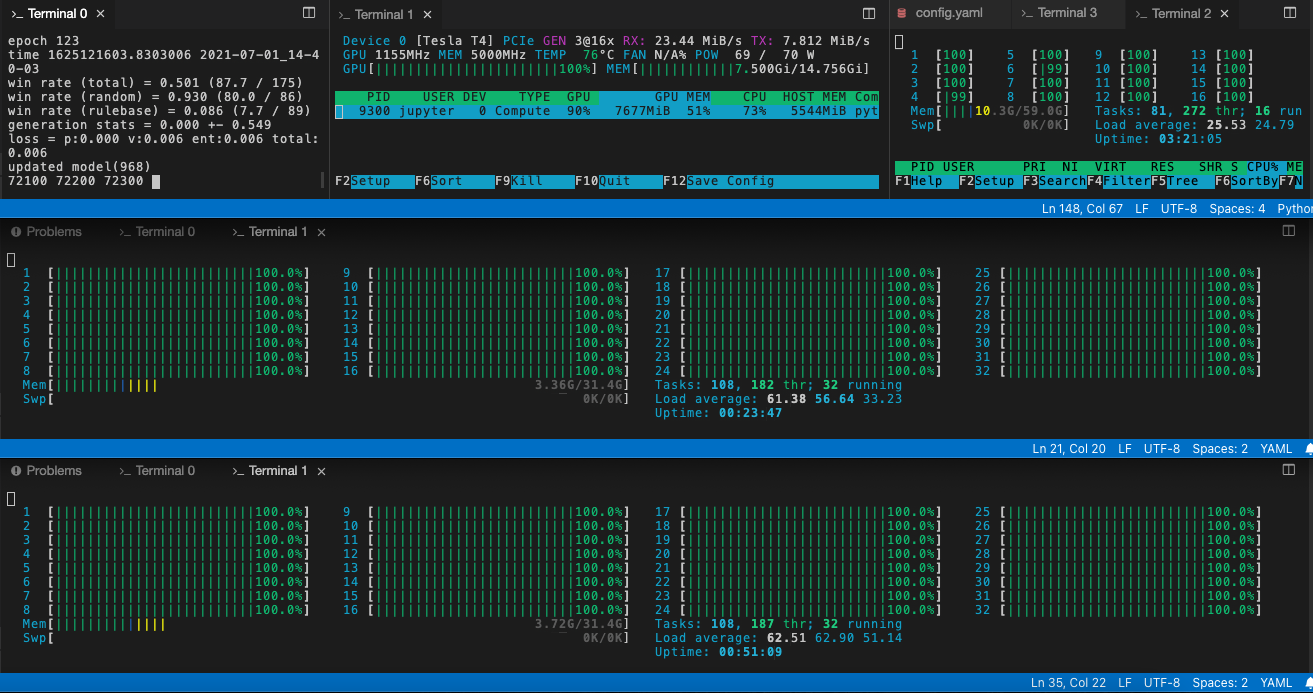
\includegraphics[width=\textwidth]{images/training-resources.png}
\caption{Screenshot of Training Setup}
\label{figure_training_setup}
\end{figure}

The actors are run on two preemptible \verb|e2-highcpu-32| instances. As the actors do not require much memory, a \verb|highcpu| instance subclass is chosen for some cost savings. As training is decentralised, the instances are also preemptible to save up to 80\% of the cost. The actors cost around US\$0.71 per hour.

The learner is run on one \verb|n1-highmem-16| instance with a T4 GPU. We need a instance with high memory to store the large number of episodes for experience replay. The instance will cost around \$1.30 per hour \cite{website_google_compute_engine_pricing}.

It takes 24 hours to train the PubHRL model with 2.1 million generated episodes over 4200 epochs. The training curve is shown in Figure \ref{figure_alt_arch}. The \$300 Google Cloud welcome credits has helped to alleviate our computation costs.

\subsection{Alternate Model Architectures and Hyperparameters}
\label{subsection_alt_model_arch_hyper_param}

Modifying the model architecture has the potential to improve the model. A model can be considered to have improved if it provides better suggestions on which move to take, or takes a shorter time to make an inference.

There is a performance-cost trade-off when we design the model architecture. A larger model may have a better performance, however, a larger model takes a longer time for inference. The larger model with a better performance may not produce a better agent as the depth of the tree search is shallower. 

This section documents the different model architectures that we have tried. Figure \ref{figure_alt_arch} shows the training curve against the default rule-based agent by Kaggle \cite{repo_kaggle_environments}. The objective function value is defined to be 1.00 if the model gets a first place, 0.67, 0.33 and 0.00 if the model gets second, third or fourth place. The score plotted is the average of the 500 games simulated per epoch.

\begin{figure}[h!]
\centering
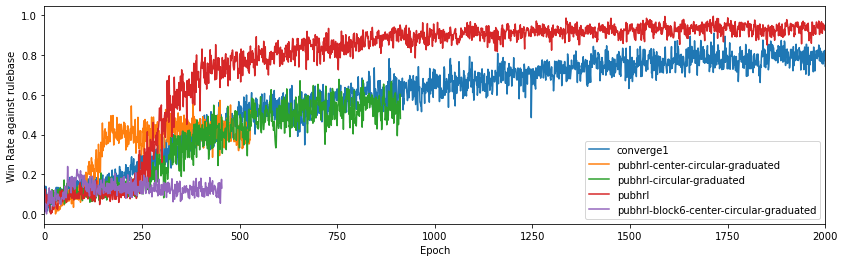
\includegraphics[width=\textwidth]{images/model-variations.png}
\caption{Training Trajectories of Various Models}
\label{figure_alt_arch}
\end{figure}


\verb|pubhrl|\newline
We attempt to reproduce the training with the original model architecture shared by HandyRL. We use the training hyperparameters shared by the authors \cite{discussion_PubHRL_parameters}.
Notably, the performance of the model only start to significantly improve after the 250th epoch. This suggests the volatile nature of training reinforcement learning models.

\verb|pubhrl-circular-graduated|\newline
In the input to the original model, the orientation of the body is not well-defined. The main change in this variant is to modify the input to better define the orientation of the body. Instead of having binary input for the four body slices, we used \verb|2/math.log(i,2)| where \verb|i| is $4$ if it is the tail, and an increment for every unit of body from the tail. The tail will have a value of $1$, and it decreases asymptotically to zero further away from down the tail. The intention is to encode the arrangement of the body in the hopes that the model will learn the arrangement. A high value implies that the location will soon be unoccupied.

We also changed the code that builds the convolutional layers, even though the behaviour is the same. The original PubHRL code makes copies of the array to pad feature matrix. We avoided the copying by using PyTorch \verb|nn.Conv2d| with the initialisation parameter \verb|padding_mode| as \verb|"circular"|.

\verb|pubhrl-center-circular-graduated|\newline
In addition to the previous model, we transpose the input such that the head is always at the coordinate \verb|(0,0)|. While we a steep improvement in training objective score at the at around the 100th epoch, the performance plateaued.

\verb|pubhrl-block6-center-circular-graduated|\newline
In addiditon to the previous model, we attempt to train a smaller model and see if is possible to achieve comparable performance. The original model architecture has 12 layers of Torus Blocks, we have reduced to 6 in this experiment. However, we have given up on the training as we do not see the model performance improve at the 400th epoch.

\verb|converge-1|\newline
This model architecture is inspired by the ResNet architecture \cite{paper_resnet}. After every residual block the the ResNet, a pooling operation is applied which reduces the dimension while increasing the number of channels. This allows more abstract features to be learnt. While the training trajectory is promising, it does not perform better at the training objective.

The alternate model architectures we have experimented did not produce superior performance on the training objective compared to the original model shared by the authors. Therefore, in our future experiments, we continued used the original architecture. After the competition, one of the top teams reported that drastically different models, such as multi-layer perceptrons and minified versions of ResNet and EfficientNet, have not shown benefit  \cite{sharing_robga}.

\subsection{Training against Different Agents}
\label{subsection_training_against_different_agents}

Instead of modifying the model architecture, there is an opportunity to improve the performance of the model by changing the agents that the model is trained against. In the Figure \ref{figure_alt_arch}, the model is trained against the default rule-based agent provided by the repository. In this subsection, we trained the model against better rule-based agents shared by other participants on Kaggle. The training logs and the code to plot the logs are available in an repository described in Section \ref{subsection_training_logs}.

As we use the same model architecture as PubHRL shared by the HandyRL authors, we begin our training from their pretrained parameters.
\newline

\begin{figure}[h!]
\centering
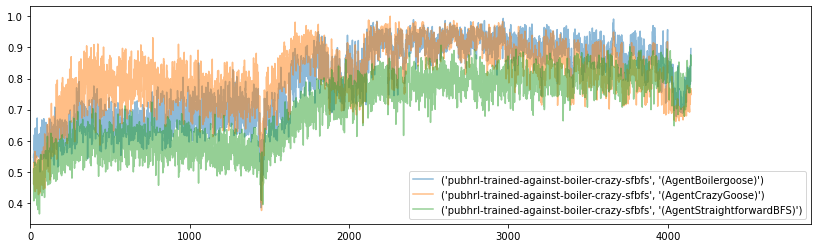
\includegraphics[width=\textwidth]{images/model-against-boiler-greedy-bfs.png}
\caption{Training Trajectories against three rule based agents}
\label{figure_assorted}
\end{figure}


\verb|pubhrl-trained-against-boiler-crazy-sfbfs|\newline
We finetune the PubHRL parameters by training against three agents - namely 
Boilergoose \cite{notebook_boilergoose}, Crazy Goose \cite{notebook_crazy_goose} and Straightforward BFS \cite{notebook_agents_comparison}. These three agents are selected from because their general good performance against other rule-based agents and against PubHRL \cite{notebook_agents_comparison}. 

The trajectory of the training objective is plotted in Figure \ref{figure_assorted}. As we use the pretrained parameters, the training objective value starts at around 0.5, rather than zero when trained from scratch. There is an unexplained dip in training objective value at around 1500th epoch, after which the model improved its performance to some peak. However, at the end of training, the training objective value declined.

\begin{figure}[h!]
\centering
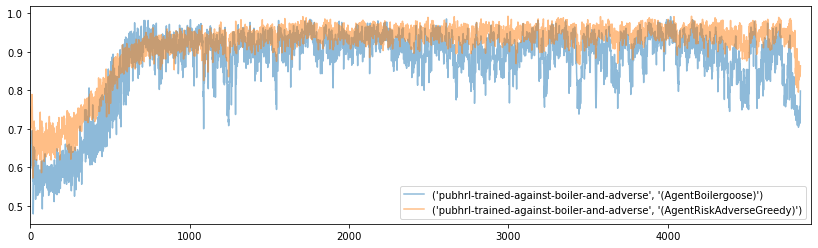
\includegraphics[width=\textwidth]{images/model-against-greedy-adverse.png}
\caption{Training Trajectories against two rule based agents}
\label{figure_greedy_adverse}
\end{figure}

\verb|pubhrl-trained-against-boiler-and-adverse|\newline
We decide the reduce the number of agents that we are training against. We choose to train the model against Boilergoose \cite{notebook_boilergoose} and Risk Adverse Greedy Goose \cite{notebook_risk_adverse_greedy} because of their very different strategies but similarly high performance. We managed to train the model to score at around 0.9 against both models. After 4000 epochs, the training objective value declined. Eventually, we used the model checkpoint at the 3600 epoch.


\subsection{Weaknesses of the Neural Network Model}
\label{subsubsection_nn_weakness}

The neural network may produce suggested moves that are certain to be bad. We show two examples from the neural network fine-tuned by us.

\subsubsection{Tail Strike}
\label{subsubsection_tail_strike}

It is usually permissible to enter the location of the tail of another geese, because the location is unoccupied as the other geese moves to the next step. However, if the other geese happens to capture a food in the next step, the location of the tail is not unoccupied. This results in the elimination of the geese. Due to the rarity of such occurrence, the model might not be able to train on this scenario well enough.

\begin{figure}[h!]
\centering
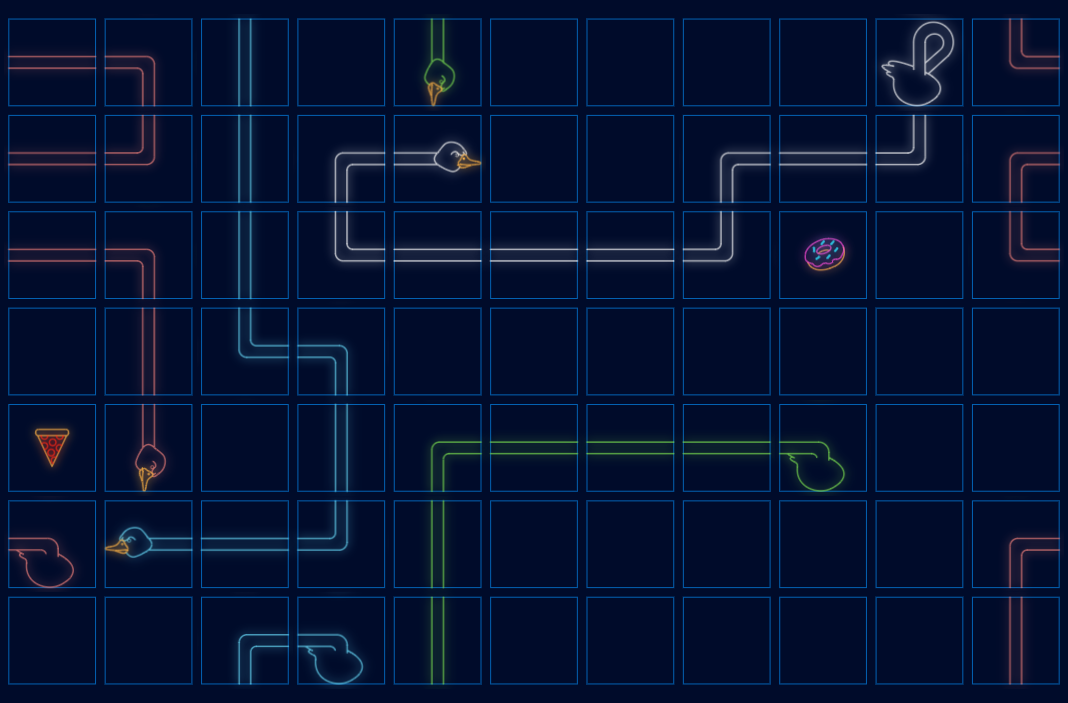
\includegraphics[width=\textwidth]{images/scenario-tail-strike.png}
\caption{Scenario of Tail Strike (Our agent is blue)}
\label{figure_tail_strike}
\end{figure}

Figure \ref{figure_tail_strike} shows a scenario of a tail strike. Our agent blue, is considering two feasible moves, left or down.

\begin{table}[h!]
\begin{tabular}{lllll}
Direction                   & Up     & Down   & Left   & Right  \\
Model Inference Probability & 0.0000 & 0.0431 & 0.9569 & 0.0000
\end{tabular}
\end{table}

In this scenario, the model make a strong suggestion to step into the location of the tail of probability 0.9569. However, the only move that red agent can make to survive is to go left to eat the food. If we follow the action suggested by the model, our agent will be eliminated.

\subsubsection{Length Ignorance}
\label{subsubsection_length_ignorance}

When two heads collide, both geese will be eliminated at the same time. The geese with the longer length will get a higher position, while the geese with the shorter length will be relegated to the lower position. However, surviving geese will be ranked better than the pair of geese which collided head-on.

\begin{figure}[h!]
\centering
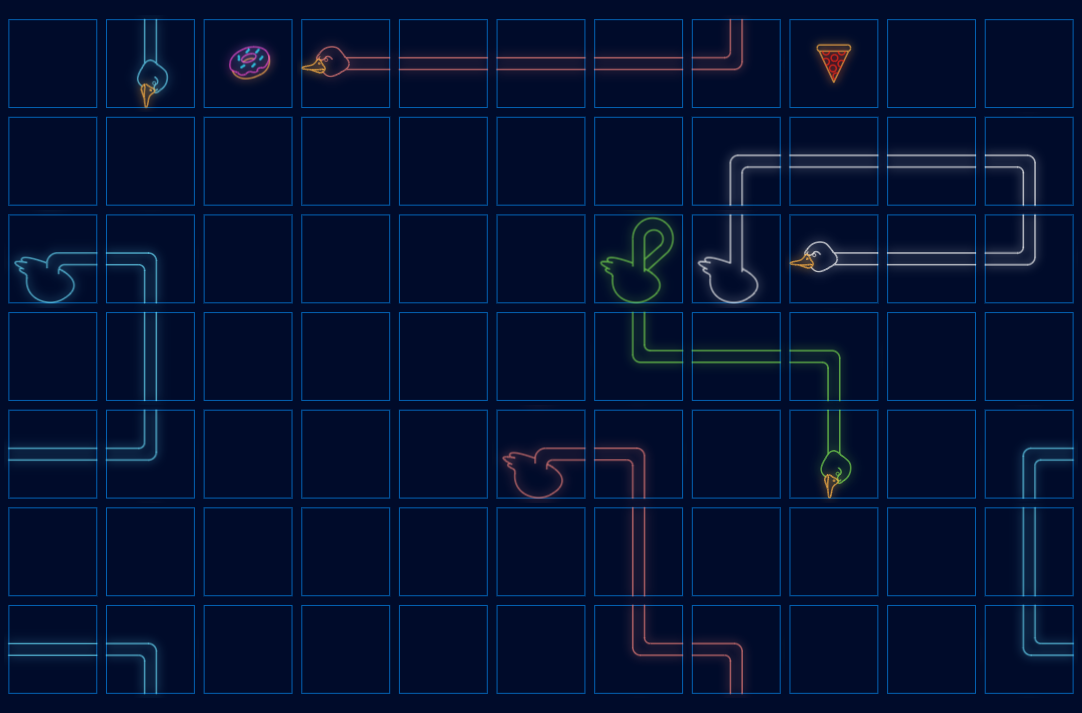
\includegraphics[width=\textwidth]{images/scenario-length-ignorance.png}
\caption{Scenario of Length Ignorance (Our agent is red)}
\label{figure_length_ignorance}
\end{figure}

Figure \ref{figure_length_ignorance} shows a scenario of a length ignorance. Our agent red, is considering three feasible moves. The agent can move left to capture the food, or move up or down to avoid the food. Our red agent is 10 units long, one unit shorter than our rival which is 11 units long. If we collide with the blue agent over the food, we get the worst possible outcome.

\begin{table}[h!]
\begin{tabular}{lllll}
Direction                   & Up     & Down   & Left   & Right  \\
Model Inference Probability & 0.0007 & 0.0031 & 0.9962 & 0.0000
\end{tabular}
\end{table}

Neural Network models may also make other move suggestions that may result in the worst possible outcome. A top team \cite{sharing_robga} shared about how they use rule-based oversight to avoid getting into traps and corridors, as well as trapping other agents.


% random rollouts?

% We tried to self train but it does not really work. 